% Options for packages loaded elsewhere
\PassOptionsToPackage{unicode}{hyperref}
\PassOptionsToPackage{hyphens}{url}
%
\documentclass[
]{article}
\title{GENNBIO COURSES}
\author{}
\date{\vspace{-2.5em}}

\usepackage{amsmath,amssymb}
\usepackage{lmodern}
\usepackage{iftex}
\ifPDFTeX
  \usepackage[T1]{fontenc}
  \usepackage[utf8]{inputenc}
  \usepackage{textcomp} % provide euro and other symbols
\else % if luatex or xetex
  \usepackage{unicode-math}
  \defaultfontfeatures{Scale=MatchLowercase}
  \defaultfontfeatures[\rmfamily]{Ligatures=TeX,Scale=1}
\fi
% Use upquote if available, for straight quotes in verbatim environments
\IfFileExists{upquote.sty}{\usepackage{upquote}}{}
\IfFileExists{microtype.sty}{% use microtype if available
  \usepackage[]{microtype}
  \UseMicrotypeSet[protrusion]{basicmath} % disable protrusion for tt fonts
}{}
\makeatletter
\@ifundefined{KOMAClassName}{% if non-KOMA class
  \IfFileExists{parskip.sty}{%
    \usepackage{parskip}
  }{% else
    \setlength{\parindent}{0pt}
    \setlength{\parskip}{6pt plus 2pt minus 1pt}}
}{% if KOMA class
  \KOMAoptions{parskip=half}}
\makeatother
\usepackage{xcolor}
\IfFileExists{xurl.sty}{\usepackage{xurl}}{} % add URL line breaks if available
\IfFileExists{bookmark.sty}{\usepackage{bookmark}}{\usepackage{hyperref}}
\hypersetup{
  pdftitle={GENNBIO COURSES},
  hidelinks,
  pdfcreator={LaTeX via pandoc}}
\urlstyle{same} % disable monospaced font for URLs
\usepackage[margin=1in]{geometry}
\usepackage{longtable,booktabs,array}
\usepackage{calc} % for calculating minipage widths
% Correct order of tables after \paragraph or \subparagraph
\usepackage{etoolbox}
\makeatletter
\patchcmd\longtable{\par}{\if@noskipsec\mbox{}\fi\par}{}{}
\makeatother
% Allow footnotes in longtable head/foot
\IfFileExists{footnotehyper.sty}{\usepackage{footnotehyper}}{\usepackage{footnote}}
\makesavenoteenv{longtable}
\usepackage{graphicx}
\makeatletter
\def\maxwidth{\ifdim\Gin@nat@width>\linewidth\linewidth\else\Gin@nat@width\fi}
\def\maxheight{\ifdim\Gin@nat@height>\textheight\textheight\else\Gin@nat@height\fi}
\makeatother
% Scale images if necessary, so that they will not overflow the page
% margins by default, and it is still possible to overwrite the defaults
% using explicit options in \includegraphics[width, height, ...]{}
\setkeys{Gin}{width=\maxwidth,height=\maxheight,keepaspectratio}
% Set default figure placement to htbp
\makeatletter
\def\fps@figure{htbp}
\makeatother
\setlength{\emergencystretch}{3em} % prevent overfull lines
\providecommand{\tightlist}{%
  \setlength{\itemsep}{0pt}\setlength{\parskip}{0pt}}
\setcounter{secnumdepth}{-\maxdimen} % remove section numbering
\usepackage{pdfpages}
\ifLuaTeX
  \usepackage{selnolig}  % disable illegal ligatures
\fi

\begin{document}
\maketitle

\begin{center}\rule{0.5\linewidth}{0.5pt}\end{center}

\begin{longtable}[]{@{}lll@{}}
\toprule
1. Plant Biotechnology (Laboratory) & Quantity & Price \\
\midrule
\endhead
Introduction to in vitro technics & 1 & 45.00 USD \\
Plant culture medium formulation & 1 & 70.00 USD \\
Anther culture & 1 & 70.00 USD \\
Aclimatization & 1 & 45.00 \\
\bottomrule
\end{longtable}

\begin{center}\rule{0.5\linewidth}{0.5pt}\end{center}

\begin{longtable}[]{@{}lll@{}}
\toprule
2. Diseño Experimental (WiFi zone) & Quantity & Price \\
\midrule
\endhead
DCA, DBCA, DCL, Parcelas, Arreglos factoriales & 1 & 45.00 USD \\
Análisis de experimentos y uso de software R & 1 & 70.00 USD \\
Análisis de experimentos y uso de software Minitab & 1 & 70.00 USD \\
Análisis de datos moleculares & 1 & ask for \\
\bottomrule
\end{longtable}

\begin{center}\rule{0.5\linewidth}{0.5pt}\end{center}

\begin{longtable}[]{@{}lll@{}}
\toprule
3. Econometría (WiFi zone) & Quantity & Price \\
\midrule
\endhead
Proyecciones simples & 1 & 30.00 USD \\
Proyecciones múltiples & 1 & 45.00 USD \\
Valoración y riesgo & 1 & 45.00 USD \\
Modelos estadísticos & 1 & 70.00 USD \\
\bottomrule
\end{longtable}

\begin{center}\rule{0.5\linewidth}{0.5pt}\end{center}

\begin{longtable}[]{@{}lll@{}}
\toprule
4. Bioinformatics (Laboratory and WiFi zone) & Quantity & Price \\
\midrule
\endhead
Genomics repositories & 1 & 30.00 USD \\
Sequence homology & 1 & 45.00 USD \\
Web sites & 1 & 70.00 USD \\
Synbio & 1 & 70.00 USD \\
Genetic transformation & 1 & 100.00 USD \\
\bottomrule
\end{longtable}

\begin{figure}
\centering
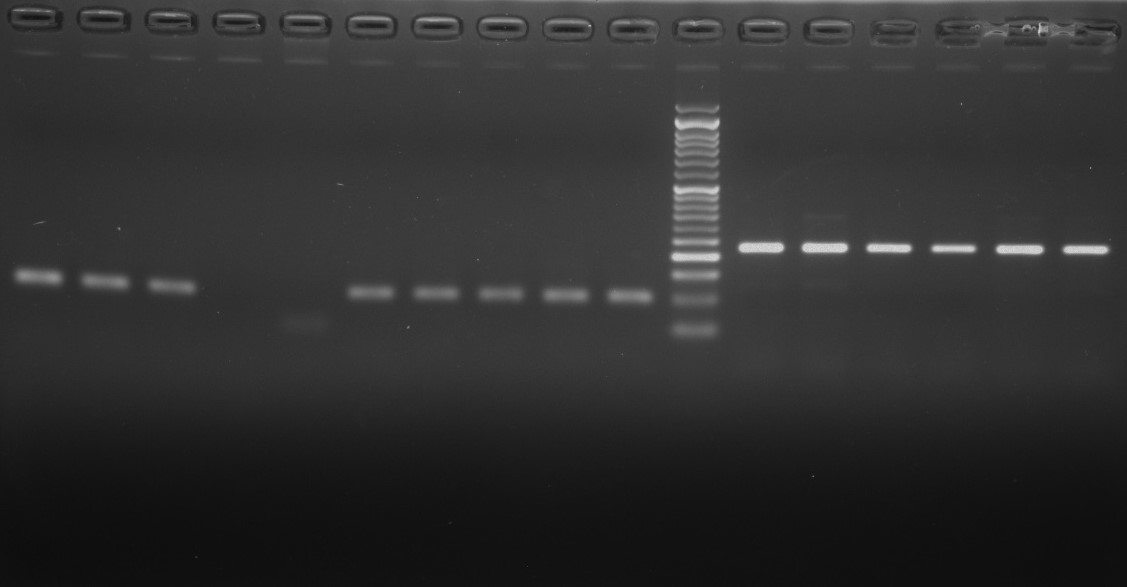
\includegraphics[width=0.1\textwidth,height=\textheight]{C:/Users/Dell/Desktop/GENNBIO.github.io/Gel_NN.jpg}
\caption{\emph{Analysis.}}
\end{figure}

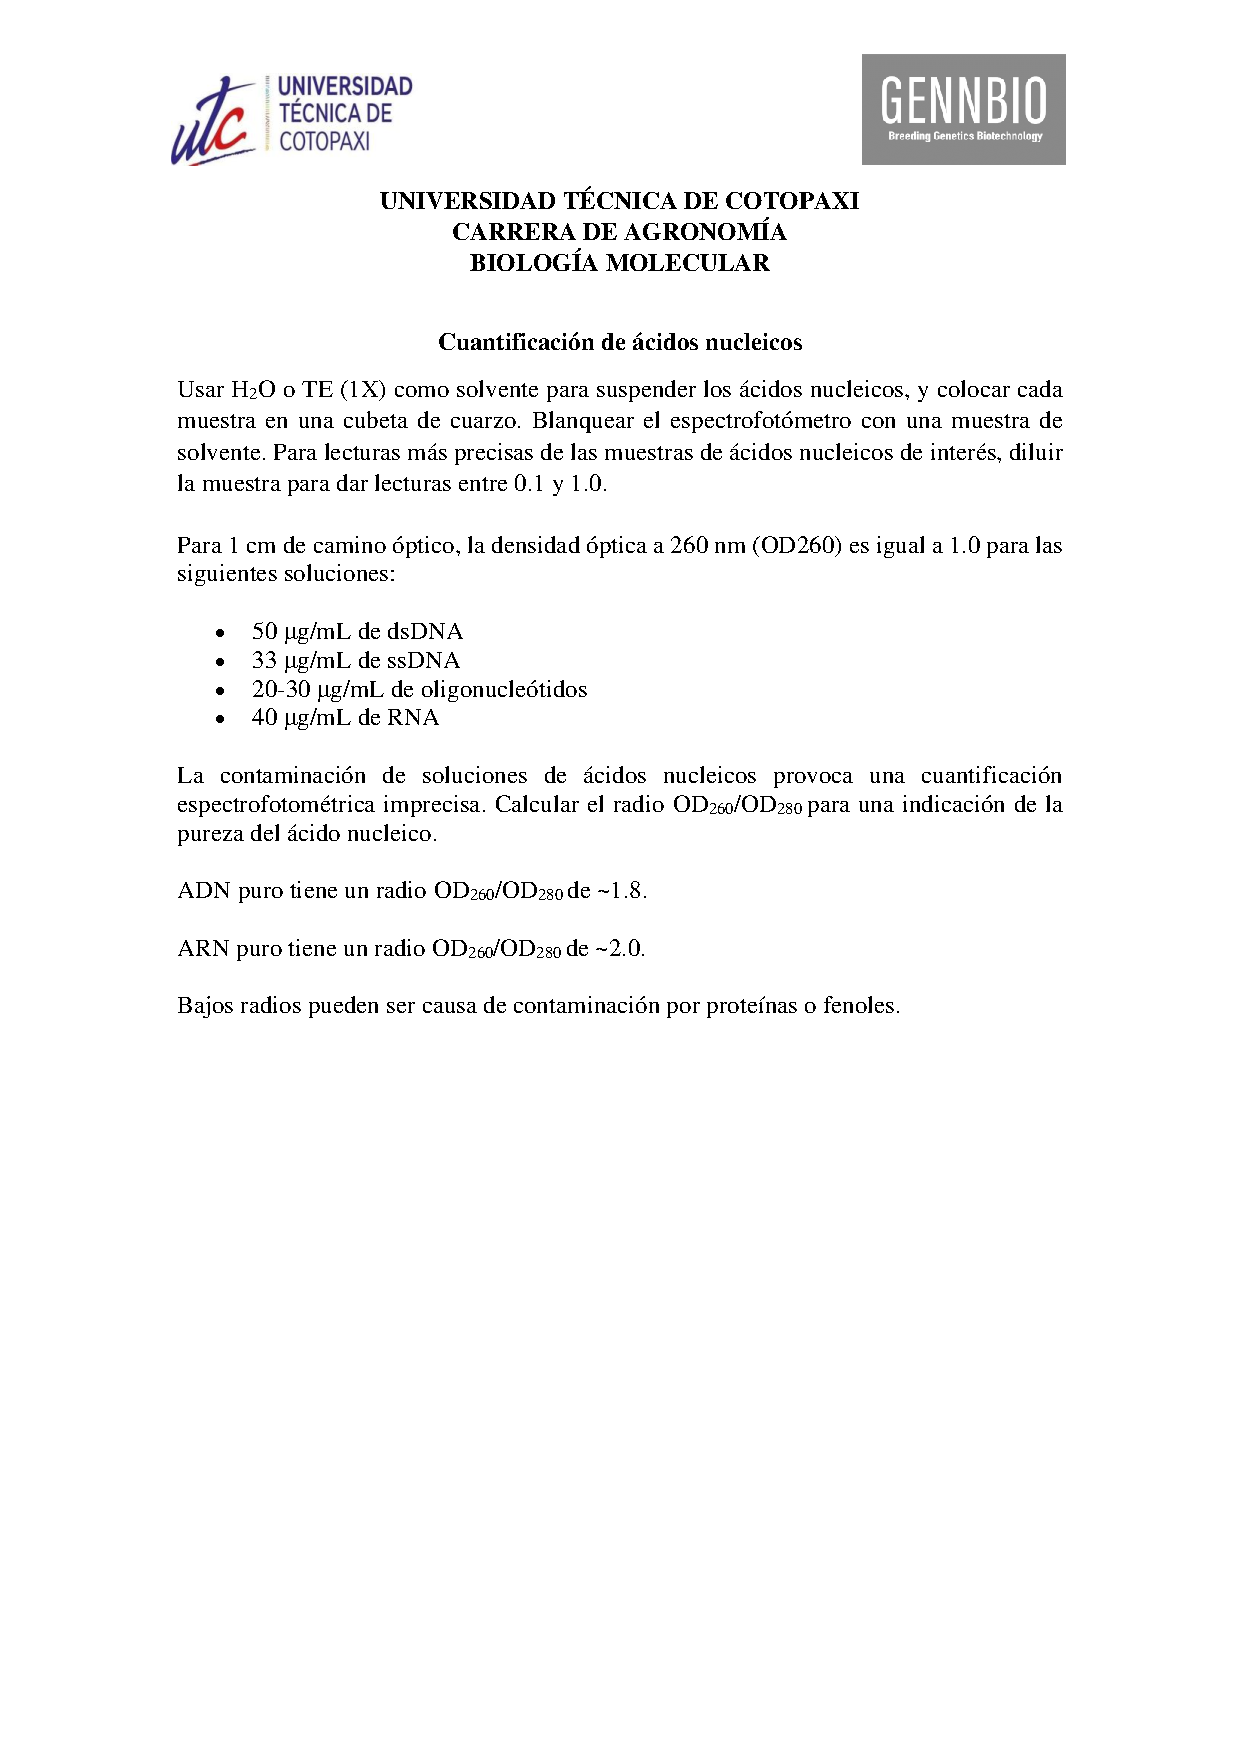
\includepdf[pages=-]{Cuantificación_NN.pdf}

\end{document}
